\documentclass[a4paper,11pt]{article}
\usepackage[utf8]{inputenc}
\usepackage[czech]{babel}
\usepackage{listings}
\usepackage{url}
\usepackage{amsmath}
\usepackage{graphicx}
\usepackage{hyperref}
\usepackage{indentfirst}


\title{Závěrečná zpráva k semestrální práci\\
		YouTube reranking\\}
\vfill
\author{Petr Kubín\\
Herbert Waage\\
FIT ČVUT\\}
\date{\today}

\begin{document}

\maketitle
\newpage

\tableofcontents
\newpage

\section{Popis projektu}
\subsection{Zadání práce}
\par{Cílem projektu je vytvoření aplikace umožňující vylepšené vyhledávání ve fotografiích uložených na serveru \href{www.youtube.com}{Youtube}. Youtube poskytuje aplikační rozhraní umožňující získat prakticky libovolná data o videích, která jsou
přístupna i z oficiálního webového rozhraní. Cílem projektu je tedy aplikace, která umožní vyhledávání na
Youtube založené na klíčových slovech, stejně jako je tomu na Youtube nyní, ale navíc bude možné zadat
sekundární vyhledávání na libovolná metadata.}
\subsection{Vstup}
\par{Klíčové slovo, sada hodnot metadat pro setřídění a počet výsledků (omezení velikosti výstupu).}
\subsection{Výstup}
\par{Videa, jejichž popis odpovídá klíčovému slovu. V levém sloupci jsou videa v původním nepřerankovaném pořadí, v pravém sloupci jsou videa setříděna podle vzdálennosti ke zvoleným metadatům.}

\section{Způsob řešení}
\subsection{Komunikace s Youtube API}
\par Začátek komunikace s Youtube API probíhá zadáním dotahu do formuláře, odkud nám Youtube vrátí veškerá videa odpovídající hledanému výrazu s omezením maximálního počtu videí. Zde vezmeme každé video a pomocí parseru zjistíme identifikátor videa, což je řetězec za watch?v=, dlouhý max 12 znaků a omezený buď koncem řetězce nebo znakem \&. Po získání identifikátoru videa jsme přešli ke stažení metadat. 

\subsection{Identifikace záznamů odpovídajících klíčovému slovu}

\subsection{Získání metadat k (identifikovaným) záznamům}
\par Pro získání jsme použili curl, neboť standartní HTTP požadavek není na školním serveru webdev, kde je naše aplikace umístěna, povolen. Pro začátek komunikace je potřeba mít vlastní API klíč, který umožní identifikovat náš program oproti YouTube API a tím dokončit požadavek. Pro samotné získání metadat jsme využili \url{https://www.googleapis.com/youtube/v3/videos?id=".$id."&key=".API_KEY."&part=snippet,statistics,contentDetails,recordingDetails}. Kde proměnná \$id je identifikátor videa získaný rozparsováním url adresy a API\_KEY je již zmiňovaný unikátní klíč.

\subsection{Výpočty různých typů vzdáleností}
\par V naší aplikaci se vyskytuje několik datových typů: řetězec, číslo, GPS, datun. Pro každý datový typ jsme museli použít správný výpočet vzdálennosti. Pro číselné datové typy jsme použili euklidovskou vzdálennost. GPSky jsme porovnali pomocí Great circle distance, která přesně určí nejmenší vzdálennost na naší zeměkouli.
\par Pro typ řetězec, který je použit u jména Autora videa, jsme naprogramovali Levenshteinovu(editační) vzdálenost, která reprezentuje počet operací nutných k převedení jednoho řetězce na druhý.

\subsection{Třídění podle daných atributů}
\par // TODO

\subsection{Webový interface}
\par Naše aplikace je nasazena na \href{http://webdev.fit.cvut.cz/~kubinpe5/MI-VMW/}{serveru webdev}. Pro styly jsme použili framework bootstrap, který umožňuje efektivní formátovaní webových elementů. 
\begin{figure}[h]
	\centering
	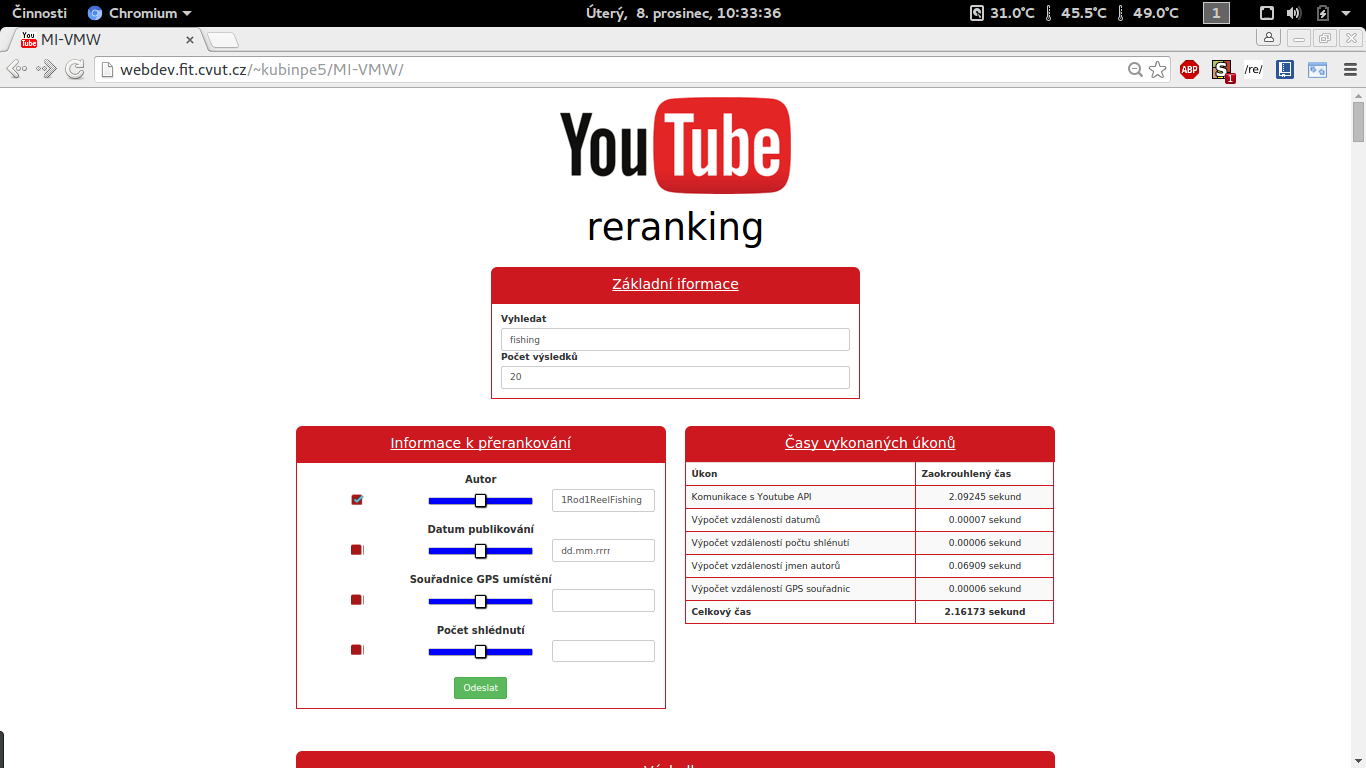
\includegraphics[width=\textwidth]{obrazova_priloha/sample_project.png}
	\caption{Náhled aplikace}
\end{figure}

\section{Příklad výstupu}
\par Výstup se skládá ze dvou sloupců. Levý sloupec reprezentuje staré uspořádání dat a pravý sloupec nové pořadí dle uživatelského vstupu v sekci informace k přerankování. Celkový počet videí je omezen znovu uživatelským vstupem. V následující kapitole bude zmíněno testování rychlosti.
\begin{figure}[h]
	\centering
	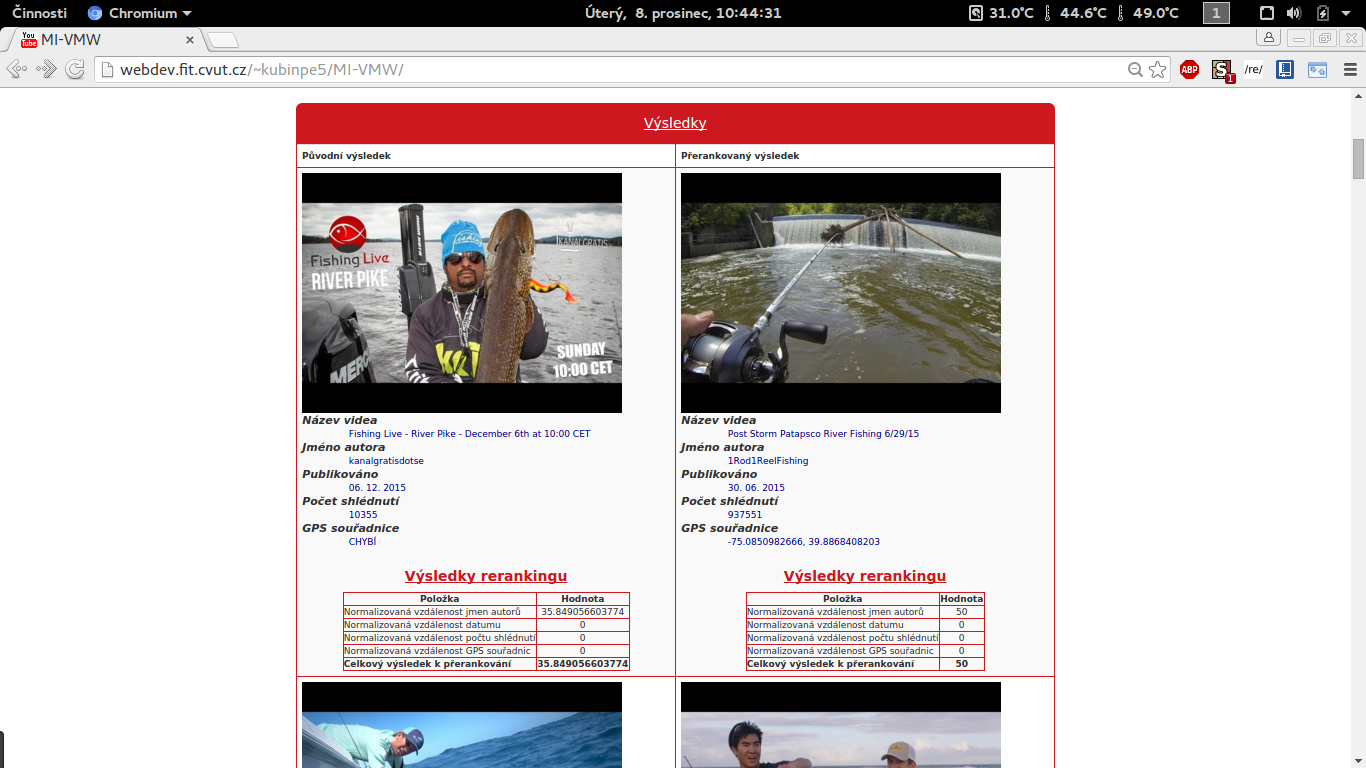
\includegraphics[width=\textwidth]{obrazova_priloha/sample_result.png}
	\caption{Náhled výsledku}
\end{figure}



\section{Experimentální sekce}
\par //TODO

\section{Diskuze}


\section{Závěr}


\newpage
\renewcommand{\refname}{Citace}
\begin{thebibliography}{9}
	\bibitem{YouTube API}
	Getting Started with the YouTube Data API: \textit{Google Developers} [online]. [cit. 13. 11. 2014]. 
	Dostupné z~WWW: \verb|<|\url{https://developers.google.com/youtube/v3/getting-started}\verb|>|.

\end{thebibliography}

\end{document}